\documentclass{beamer}
\usetheme{Boadilla}
\usepackage{amsmath}
\usepackage{graphicx}
\graphicspath{{../images/}}
\usepackage[backend=biber, bibencoding=utf8]{biblatex}
\addbibresource{ref.bib}

\title{Bayesball}
\subtitle{Empirical Bayesian Estimation of Batting Averages}
\author{Nick Sun}
\institute{Oregon State University}
\date{\today}


\begin{document}

\begin{frame}
\titlepage
\end{frame}

\begin{frame}{Outline}
	\tableofcontents
\end{frame}

\section{Methods}
\subsection{Batting Averages}
\begin{frame}
\frametitle{Batting Averages}
\begin{itemize}
	\item No number is more important or ubiquitous in sabermetrics than batting average. The formula is simply $\frac{\text{Hits}}{\text{At-bats}}$.
	\item Batting average is  calculated cumulatively over the season, starting at .000.
		This makes the variance of early season batting average calculations quite large.
	\item We can think of these batting averages as an estimation of $p$, a batter's true probability of getting a hit in an at-bat.
	\item Is there a ``better'' $\hat{p}$ than this?
\end{itemize}
\end{frame}

\subsection{Bayesian Methods}
\begin{frame}
	\frametitle{Empirical Bayesian Estimation}
	\begin{itemize}
		\item One of the first models we learned this quarter was a binomial model with a beta conjugate prior. Perhaps we can use this for modelling $p$?
		\item If we have a prior $\pi(p) \propto p^{\alpha-1} (1 -p)^{\beta-1}$, then our posterior distribution will be:
			$$\pi(p | AB, H) \propto p^{\alpha + H - 1} (1 - p)^{\beta + AB - H - 1}$$

			where $H$ is the number of hits and $AB$ is the number of at-bats.
	\end{itemize}
\end{frame}

\begin{frame}
	\frametitle{Empirical Bayesian Estimation}
	I had three goals with this analysis:
	\begin{enumerate}
		\item Explore some ways of finding a prior $\pi(p)$
		\item Compare the MSE of empirical Bayesian estimation and normal batting average calculations as a season progressed
		\item Compare credible and confidence intervals
	\end{enumerate}
	We will answer these questions using simulations.
\end{frame}

\subsection{Confidence intervals}
\begin{frame}
\frametitle{Credible Intervals vs. Confidence Intervals}
Bayesian estimation allows us to make bayesian credible intervals which we can compare against frequentist confidence intervals. 
\begin{itemize}
	\item \textbf{Bayesian Credible interval}: \texttt{qbeta(c(.025, .975), alpha0 + cumH, beta0 + cumAB - cumH)}
	\item \textbf{Jeffrey's interval}: \texttt{qbeta(c(.025, .975), .5 + cumH, .5 + cumAB - cumH)}
	\item \textbf{Clopper-Pearson interval}: \texttt{qbeta(.025, cumH, cumAB - cumH + 1), qbeta(.975, cumH + 1, cumAB - cumH)}
\end{itemize}
where $cumH$ and $cumAB$ are the cumulative hits and at-bats at any given point in the season.\cite{robinson}
\end{frame}

\section{Simulations}
\begin{frame}
	\frametitle{Meet our Subject}
	\begin{itemize}
		\item Michael  Conforto (aka "Scooter") is a promising right fielder for the New York Mets. He's also from good ol' OSU.
		\item His young career so far has been somewhat inconsistent, fluctuating between average to All-Star.\cite{baseballreference}
	\end{itemize}
	\vspace{.5cm}
	\begin{minipage}{.6\textwidth}
		\begin{center}
		\begin{tabular}{|| c | c | c|  c ||}
			\hline
			Season & AB & H & Batting Average \\
			\hline
			2015 & 174 & 47 & .270 \\
			2016 & 304 & 67 & .220 \\
			2017 & 373 & 104 & .279* \\
			2018 & 543 & 132 & .243 \\
			2019 & 549 & 141 & .257 \\
			\hline
		\end{tabular}
		\end{center}
	\end{minipage}
	\begin{minipage}{.38\textwidth}
		\begin{center}
		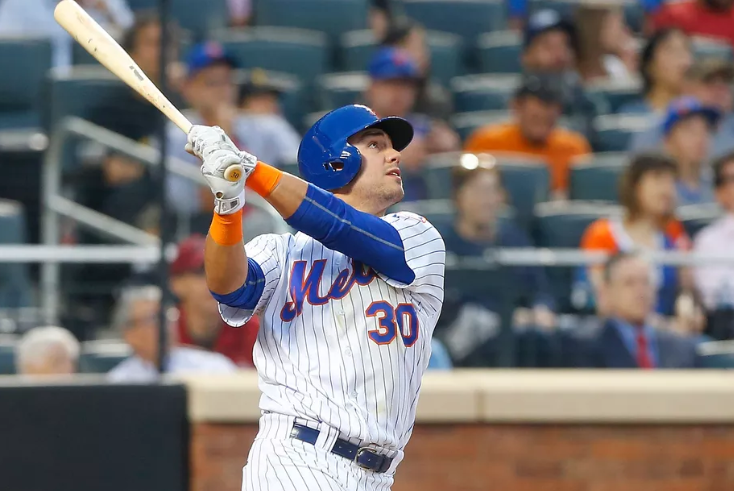
\includegraphics[width=.95\textwidth]{scooter}
		\end{center}
	\end{minipage}
\end{frame}

\begin{frame}
	\frametitle{Prior}
	A reasonable place to start with a prior is at team level.
	Below is a density histogram of all batting averages from the 2018 New York Mets.\cite{lahman}
\begin{center}
	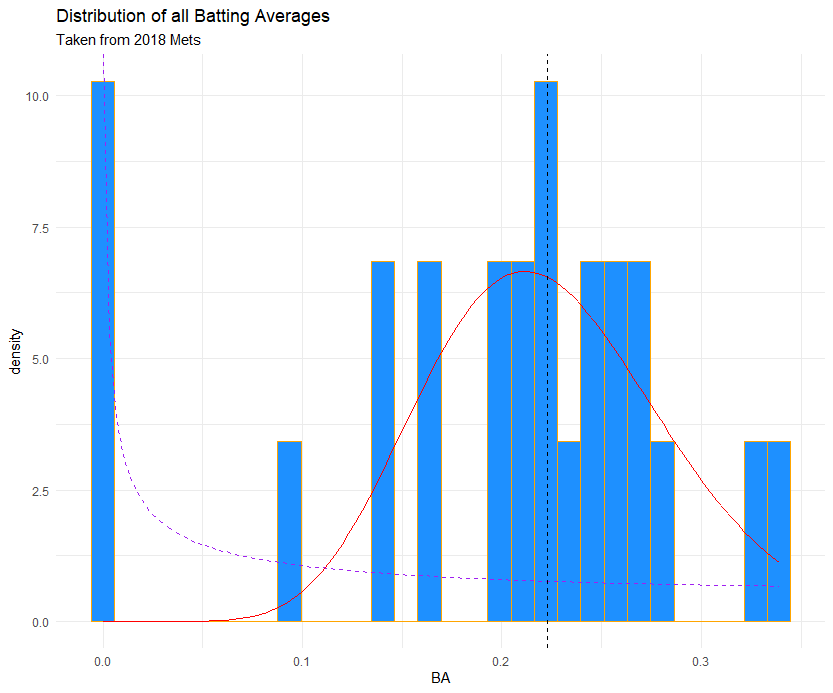
\includegraphics[height=.5\linewidth,width=.7\textwidth]{2018_mets_prior}
\end{center}
\end{frame}

\begin{frame}
	\frametitle{Prior}
	\begin{itemize}
		\item It is known that the mean of a beta distribution is given by $\frac{\alpha}{\alpha+\beta}$.
		\item We can therefore try ``shifting'' the mean of this Mets distribution by changing the value of $\alpha$ to Michael Conforto's batting average in 2018 
		\item This will also change the variance of the beta prior, but this was the method I found which worked the best.
		\item In 2018, Conforto had a batting average of .243 which gave me a prior of Beta(11.74, 36.76)
	\end{itemize}
\end{frame}

\begin{frame}
	\frametitle{Simulating the 2019 season}
	Michael Conforto had a .257 batting average in 2019. If we treat this as the true value of $p$, we can simulate 1000 2019 seasons using game logs and check the MSE of our estimates at each game in the season.
	\begin{center}
		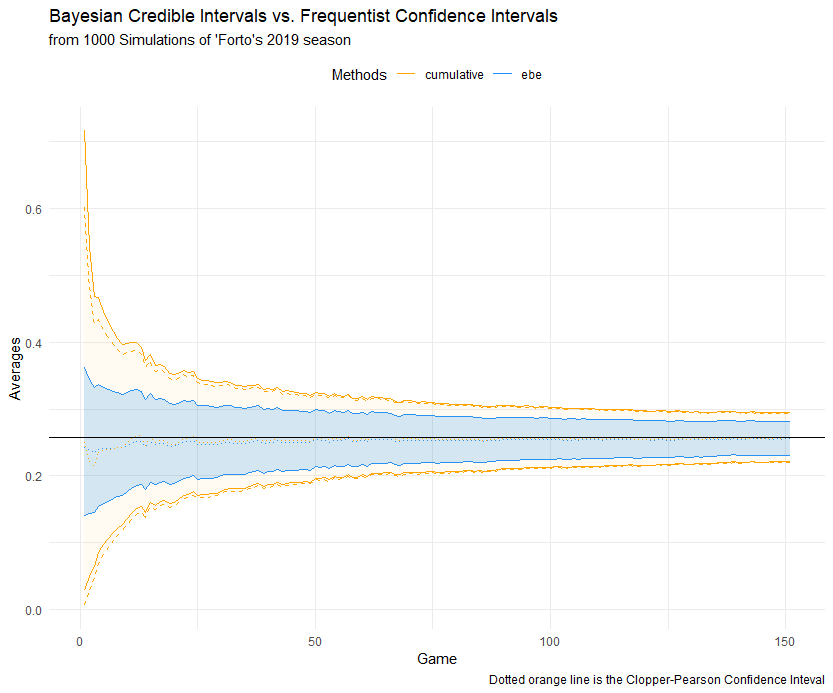
\includegraphics[height=.53\linewidth,width=.7\textwidth]{intervals_2019}
	\end{center}
\end{frame}

\begin{frame}
	\frametitle{MSE of the 2019 simulations}
	MSE is calculated as the average of the squared deviations from the true value of $p$.

	\begin{center}
		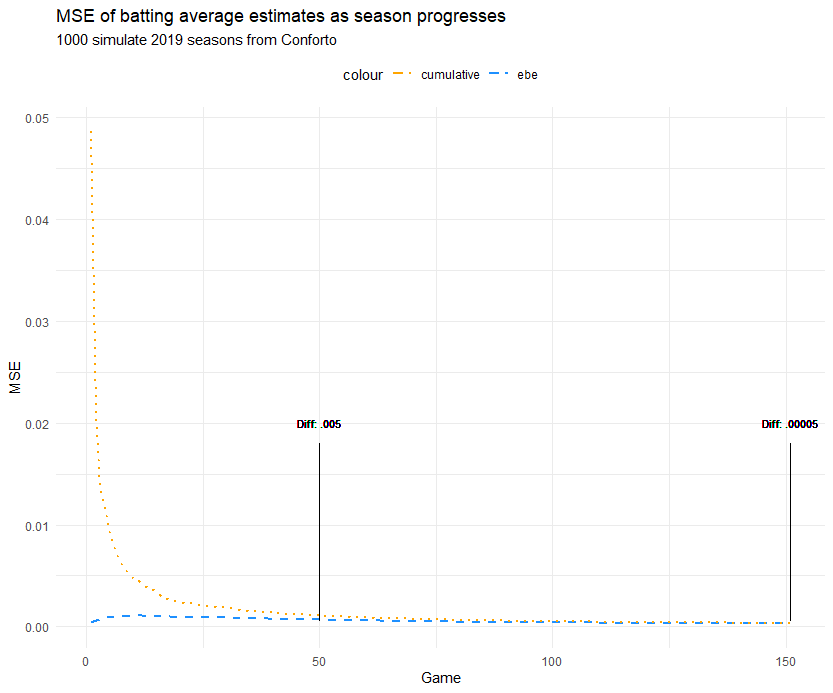
\includegraphics[height=.57\linewidth,width=.7\textwidth]{mse_2019}
	\end{center}
\end{frame}

\begin{frame}
	\frametitle{Inteval Coverage}
	For each game, I calculated the proportion in which $p$ fell within each of the three intervals.

	\begin{center}
		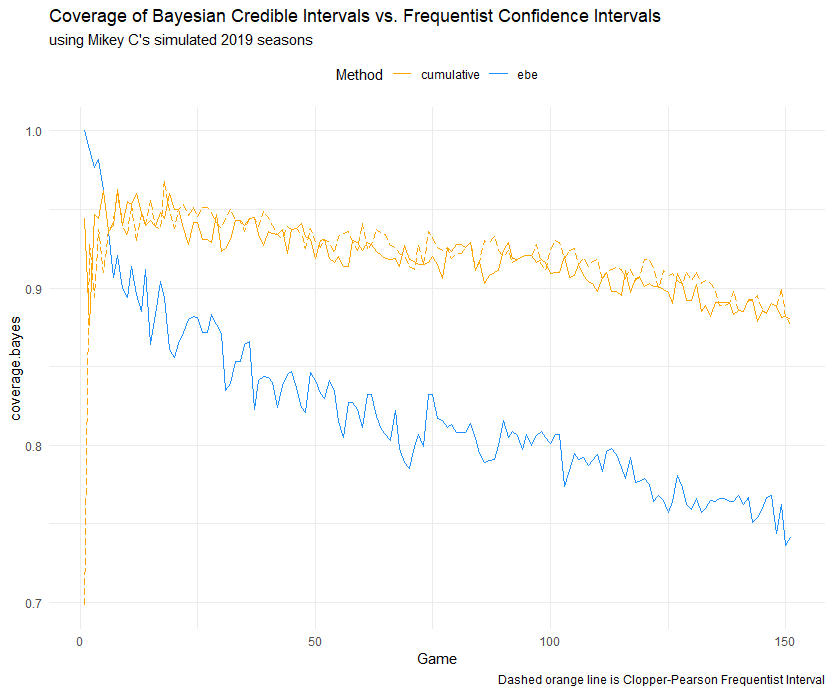
\includegraphics[height=.57\linewidth,width=.7\textwidth]{coverages_2019}
	\end{center}
\end{frame}

\begin{frame}
	\frametitle{New simulation: $p$ is drawn randomly}
	\begin{itemize}
		\item Instead of having a fixed constant $p$ for every simulated season, we will draw random a $p$ from a Beta(45.173, 117.316) distribution, representing the batting average distribution of all Mets in 2017 and adjusted to have a mean of .279
		\item The prior mean will be equal to Conforto's 2016 performance of .220
	\end{itemize}
\end{frame}

\begin{frame}
	\frametitle{Posterior distribution of parameters}
	Conforto played 109 games in 2017.
	We can plot $\alpha$ and $\beta$ for all 1000 simulated posterior distributions.
	\begin{center}
		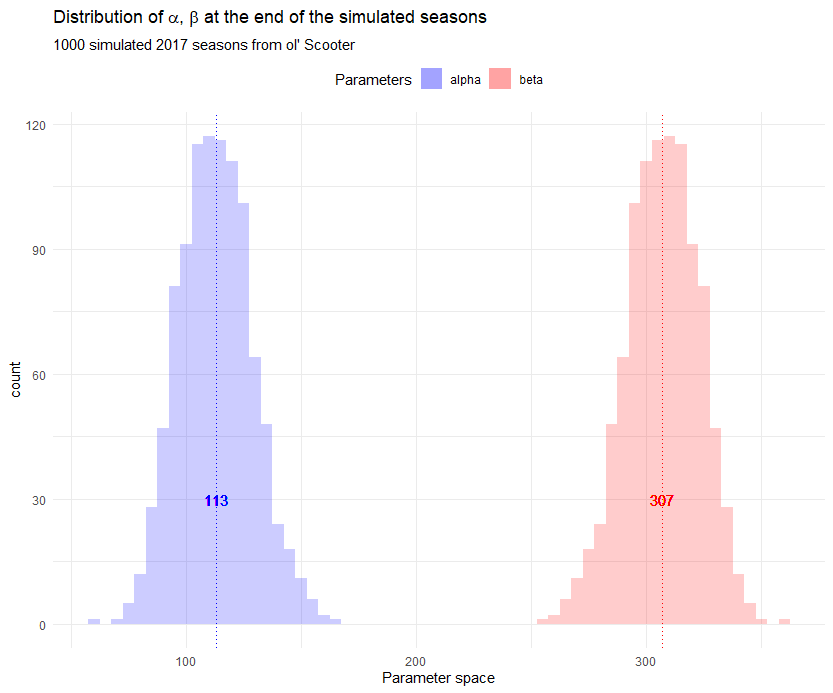
\includegraphics[height=.5\linewidth,width=.6\textwidth]{posts_2017}
	\end{center}
\end{frame}

\begin{frame}
	\frametitle{Interval Coverage}
	\begin{center}
		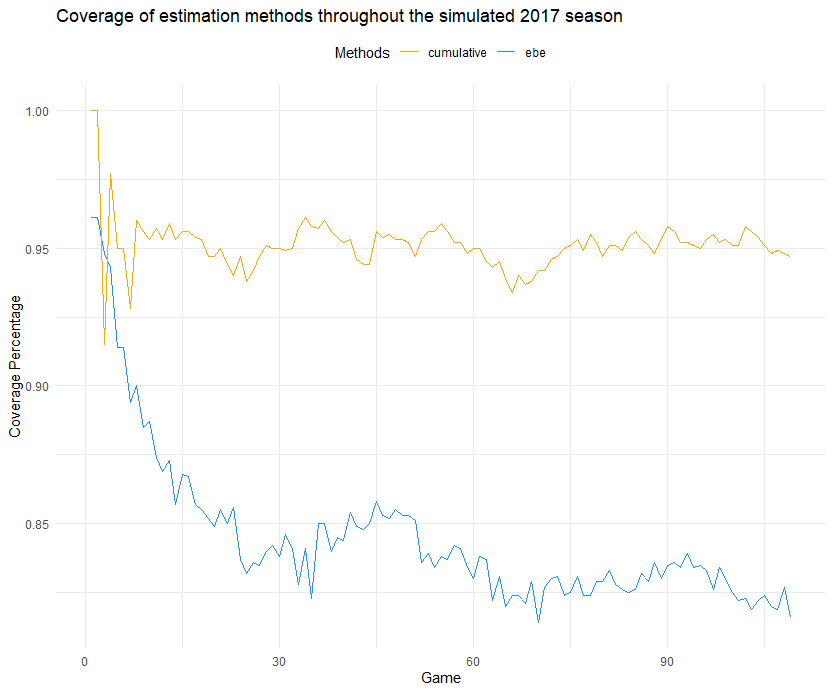
\includegraphics[height=.6\linewidth,width=.7\textwidth]{coverages_2017}
	\end{center}
\end{frame}

\begin{frame}
	\frametitle{Posterior Distribution}
	\begin{center}
		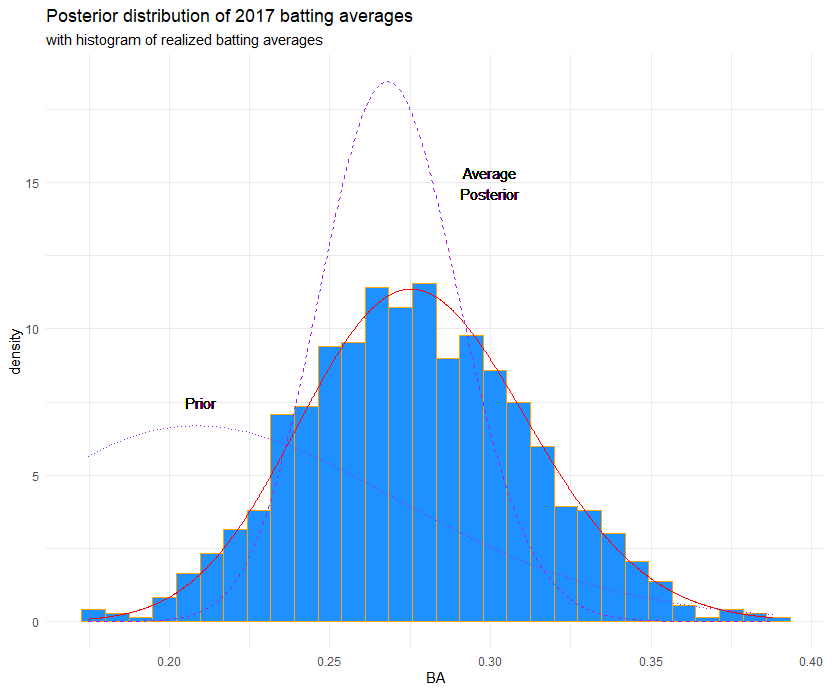
\includegraphics[height=.6\linewidth,width=.7\textwidth]{dists_2017}
	\end{center}
\end{frame}

\begin{frame}
	\frametitle{One last simulation}
	Instead of having a single $p$ for an entire season, what if $p$ was changed every day?
	This is likely a more realistic model of MLB players hitting ability.
	Again we sample random $p$ from Beta(45.173, 117.316), but this time $p$ is a vector instead of a scalar.

	\begin{center}
		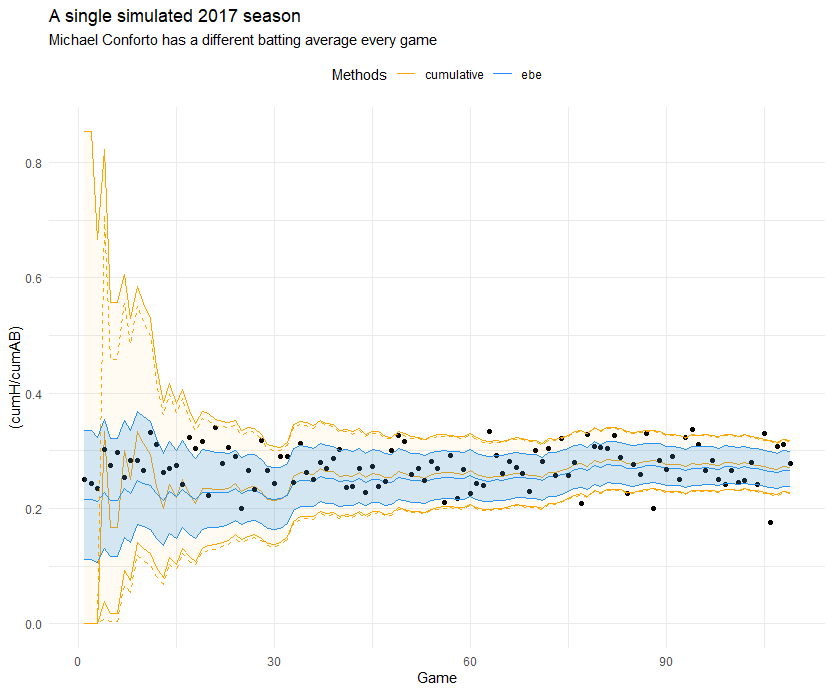
\includegraphics[height=.45\linewidth,width=.6\textwidth]{manyp_2017}
	\end{center}
\end{frame}

\begin{frame}
	\frametitle{MSE comparison}
	\begin{center}
		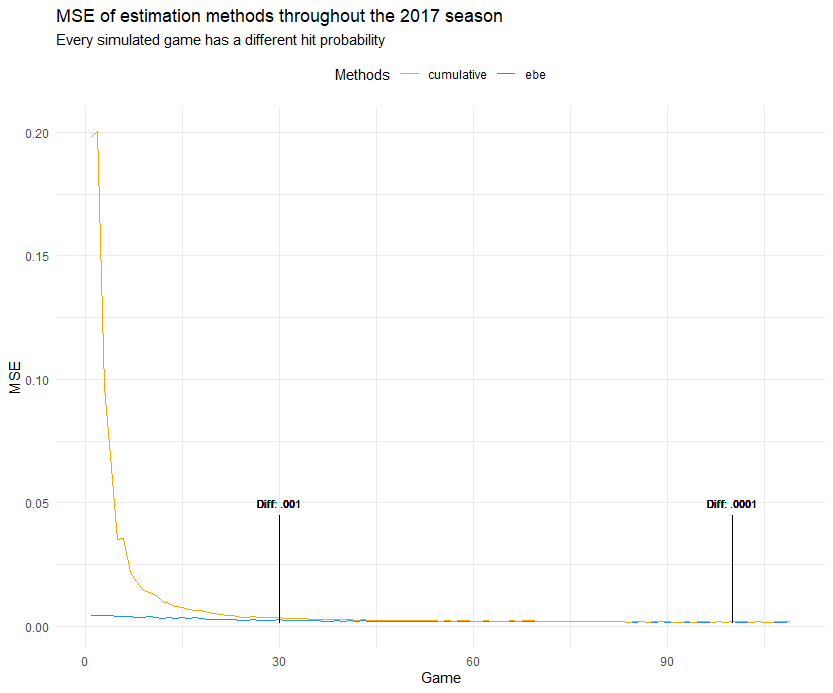
\includegraphics[height=.6\linewidth,width=.7\textwidth]{manyp_mse}
	\end{center}
\end{frame}

\section{Conclusion}
\begin{frame}
	\frametitle{Conclusion}
	\begin{itemize}
		\item Empirical Bayesian estimation with a prior based on the last season's performance had a lower MSE in all simulations and all time points, but especially in the beginning of the season
		\item Bayesian credible intervals are narrower than frequentist intervals owing to the lower variance of the posterior distribution as $\alpha$ and $\beta$ grow
		\item Both Bayesian and Frequentist intervals are too wide to be of much practical use (average width being around .1 for Bayesian intervals)
	\end{itemize}
\end{frame}

\section{References}
\begin{frame}{Reference}
\printbibliography
\end{frame}

\end{document}
